\documentclass[10pt,landscape,a4paper]{article}
\usepackage[utf8]{inputenc}
\usepackage[ngerman]{babel}
\usepackage[T1]{fontenc}
\usepackage{adigraph}
\usepackage{tikz}
\usetikzlibrary{shapes,positioning,arrows,fit,calc,graphs,graphs.standard}
\usepackage[nosf]{kpfonts}
\usepackage[t1]{sourcesanspro}
\usepackage{multicol}
\usepackage{wrapfig}
\usepackage[top=1mm,bottom=2mm,left=2mm,right=2mm]{geometry}
\usepackage[framemethod=tikz]{mdframed}
\usepackage{microtype}
\usepackage{pdfpages}
\usepackage{xfrac}
\usepackage{tikz-cd}
\usepackage{graphicx}
\newcommand*\N{\mathbb{N}}
\newcommand*\Z{\mathbb{Z}}
\newcommand*\Q{\mathbb{Q}}
\newcommand*\R{\mathbb{R}}
\newcommand*\I{\mathbb{I}}
\newcommand*\C{\mathbb{C}}
\newcommand*\PR{\mathbb{P}}
\newcommand*\poset{\mathcal{P}}

\graphicspath{ {./img/} }

\let\bar\overline

\begin{document}

\include{inhalt/def}

\small
\begin{multicols*}{4}

\section{Zahlenmengen}
{\bf Natürliche Zahlen}\\
\(\mathbb{N} = \{0,1,2,3,4,5,6,...\}\) \\
{\bf Ganze Zahlen}\\
\(\mathbb{Z} = \{...,-3,-2,-1,0,1,2,3,...\}\) \\
{\bf Rationale Zahlen}\\
\(\mathbb{Q} = \left\{ \frac{1}{2}, \frac{2}{3}, \frac{5}{4}, -\frac{3}{7}, 0, 1, -2, ... \right\}\) \\
{\bf Reele Zahlen}\\
\(\mathbb{R} = \{ -2, 0, 1.5, \sqrt{2}, \pi, e, ... \}\)

\section{Zahlensysteme}

\section{Prädikate}
Es sei n eine natürliche Zahl. Ein Ausdruck, in dem n viele
(verschiedene) Variablen frei vorkommen und der bei Belegung (=
Ersetzen) aller freien Variablen in eine Aussage übergeht, nennen wir
ein n-stelliges Prädikat.
\begin{itemize}
    \item x > 3 ist ein 1-stelliges Prädikat.
    \item x + y = z ist ein 3-stelliges Prädikat.
    \item x ist eine natürliche Zahl 1-stelliges Prädikat.
\end{itemize}
\subsection{Aussagen}
Aussagen sind 0-stellige Prädikate. Sie sind entweder wahr oder falsch.
\subsection{Quantoren}
\(\forall A\) (Allquantor aka für jedes Element)\\
\(\exists A\) (Existenzquantor aka mind. ein Element)
\subsection{Junktoren}
\(A \neg B\) (Negation)\\
\(A \wedge B\) (Konjunktion)\\
\(A \vee B\) (Disjunktion)\\
\(A \Rightarrow B\) (Implikation)\\
\(A \Leftrightarrow B\) (Äquivalenz)

\section{Gesetze und Umformungen}
Distributiv\\
\(A \wedge (B \vee C) \Leftrightarrow (A \wedge B) \vee (A \wedge C)\)\\
\(A \vee (B \wedge C) \Leftrightarrow (A \vee B) \wedge (A \vee C)\)\\

Assotiativ\\
\(A \wedge (B \wedge C) \Leftrightarrow (A \wedge B) \wedge C\)\\
\(A \vee (B \vee C) \Leftrightarrow (A \vee B) \vee C\)\\

de Morgan\\
\(\neg (A \wedge B) \Leftrightarrow \neg A \vee \neg B\)\\

\section{Aussonderung}
Ist A eine Menge und ist E(x) eine Eigenschaft (ein Prädikat), dann
bezeichnen wir mit dem Term:
\begin{equation}
    x \in A \mid E(x)
\end{equation}
Beispiel: Menge aller Geraden Zahlen:
\begin{equation}
    \{x \in \mathbb{N} \mid \exists{y} \in \mathbb{N}(x= 2y)\}
\end{equation}
\section{Ersetzung}
Ist A eine Menge und t(x) ein Ausdruck in x , dann schreiben wir
\begin{equation}
    t(A) = \{t(x) \mid x \in A\}
\end{equation}
für die Menge, die als Elemente alle Objekte von der Form t(x) mit
x \(\in\) A enthält.\\\\
Beispiel: Menge aller Quadratzahlen
\begin{equation}
    \{x^2 \mid x \in \mathbb{N}\}
\end{equation}


\section{Mengenoperationen}
\subsection{Teilmengen}
Eine Menge A ist Teilmenge einer Menge B, geschrieben $A \subseteq B$, falls alle Elemente von A auch Elemente von B sind.
Formal gilt:
\begin{equation}
    A \subseteq B \Leftrightarrow \forall{x}(x \in A \Rightarrow x \in B)
\end{equation}
Eine Teilmenge A  von B ist eine echte Teilmenge, wenn $A \neq B$ gilt. Wir schreiben $A \subset B$,
wenn A eine echte Teilmenge von B ist.

\subsubsection{Extensionalitätsprinzip}
Mithilfe der Teilmengenrelation lässt sich das Extensionalitätsprinzip wie folgt formulieren:
\begin{equation}
    A = B \Leftrightarrow A \subseteq B \wedge B \subseteq A
\end{equation}

\subsection{Potenzmengen}
die Potenzmenge $\mathcal{P}(A)$ einer Menge A ist die Menge aller Teilmengen von A. Formal gilt:
\begin{equation}
\mathcal{P}(A) \coloneqq \{B \mid B \subseteq A\}
\end{equation}
Beispiel: 
\begin{itemize}
    \item $\mathcal{P}(\{1,2\}) = \{\emptyset, \{1\}, \{2\}, \{1,2\}\}$
    \item $\mathcal{P}(\{\{a\}\}) = \{\emptyset, \{\{a\}\}\}$
\end{itemize}

Es gilt für beliebige Mengen A:
\begin{itemize}
    \item $A \in \mathcal{P}(A)$, weil jede Megne eine Teilmenge von sich selbst ist.
    \item $\emptyset \in \mathcal{P}(A)$, weil die leere Menge Teilmenge jeder Menge ist.
\end{itemize}
{\bf! Sanity-Check}: $\mathcal{P}(A)$ hat $2^{|A|}$ Elemente.
\subsection{Verenigung}
Die Verenigung von zwei Mengen beinhaltet genau die Elemente, die in mindestens einer der beiden Mengen enthalten sind. Formal gilt:
\begin{equation}
A \cup B \coloneqq \{x \mid x \in A \vee x \in B\}
\end{equation}
Beispiel:
\begin{itemize}
    \item $\{1,2,3\} \cup \{3,4,5\} = \{1,2,3,4,5\}$
    \item $\mathbb{Z} = \{-n \mid n \in \mathbb{N} \cup \mathbb{N}\}$
\end{itemize}
\begin{itemize}
    \item Möchte man beliebig viele Mengen vereinigen, d.h. alle
    Mengen, die Element einer beliebigen Menge M von Mengen
    sind, dann ist ein Existenzquantor nötig.
    \begin{equation}
        \bigcup_{A \in M} A \coloneqq \{x \mid \exists{A} \in M(x \in A)\}
    \end{equation}
    \item Sind die Mengen die man vereinigen möchte indexiert, d.H. M ist in der Form $M = \{A_i \mid i \in I\}$,
    dann verwenden wir auch die folgenden Notation:
    \begin{equation}
        \bigcup_{i \in I} A_i \coloneqq \bigcup_{A \in M} = \{x \mid \exists{i} \in I(x \in A_i)\}
    \end{equation}
\end{itemize}

{\bf Eigenschaften von $\cup$}
\begin{itemize}
    \item Kommutativität $A \cup B = B \cup A$
    \item Assoziativität $(A \cup B) \cup C = A \cup (B \cup C)$
    \item Idempotenz $A \cup A = A$
    \item $A \subseteq A \cup B$
    \item $A \subseteq B \Leftrightarrow B = A \cup B$
\end{itemize}

\subsection{Schnittmengen}
 Die Schnittmenge von zwei Mengen beinhaltet genau die Elemente, die in beiden Mengen enthalten sind:
    \begin{equation}
        A \cap B \coloneqq \{x \mid x \in A \wedge x \in B\}
    \end{equation}
Beispiel:
\begin{itemize}
    \item $\{1,2,3\} \cap \{2,3,4,5\} = \{2,3\}$
    \item $\mathbb{N} = \{r \in \mathbb{R} \mid r \geq 0\} \cap \mathbb{Z}$
\end{itemize}
\begin{itemize}
    \item Möchte man beliebig viele Mengen schneiden, d.h. alle
    Mengen, die Element einer beliebigen Menge M von Mengen
    sind, dann ist ein Allquantor nötig.
    \begin{equation}
        \bigcap_{A \in M} A \coloneqq \{x \mid \forall{A} \in M(x \in A)\}
    \end{equation}
    \item Wenn man sie indexiert haben möchte d.H. M ist in der Form $M = \{A_i \mid i \in I\}$, dann so:
    \begin{equation}
        \bigcap_{i \in I} A_i \coloneqq \bigcap_{A \in M}A = \{x \mid \forall{i} \in I(x \in A_i)\}
    \end{equation}
\end{itemize}
{\bf Eigenschaften von $\cap$}
\begin{itemize}
    \item Kommutativität $A \cap B = B \cap A$
    \item Assoziativität $(A \cap B) \cap C = A \cap (B \cap C)$
    \item Idempotenz $A \cap A = A$
    \item $A \cap B \subseteq A$
    \item $A \subseteq B \Leftrightarrow A \cap B = A $
\end{itemize}
\subsection{Disjunkte Mengen}
\begin{itemize}
    \item zwei Mengen A und B heissen {\bf disjunkt}, wenn $A \cap B = \emptyset$ gilt.
    \item Eine Menge $M = \{A_i \mid i \in I\}$ von Mengen heissen {\bf paarweise disjunkt}, 
    wenn für alle aus $i \neq j$ gilt $A_i \cap A_j = \emptyset$ folgt.
\end{itemize}
\subsection{Differenzmengen}
Sind A und B Mengen, dann bezeichnen wir mit
\begin{equation}
    A \setminus B \coloneqq \{x \in A \mid x \notin B\}
\end{equation}
die Differenz (A ohne B ) von A und B
\subsubsection{Interaktion von $\cup$,$\cap$ und $\setminus$}
Sind A, B und C beliebige Mengen, dann gilt:
\begin{itemize}
    \item De Morgan: $C \setminus (A \cap B) = (C \setminus A) \cup (C \setminus B)$
    \item De Morgan: $C \setminus (A \cup B) = (C \setminus A) \cap (C \setminus B)$
    \item Distributivität: $A \cup (B \cap C) = (A \cup B) \cap (A \cup C)$
    \item Distributivität: $A \cap (B \cup C) = (A \cap B) \cup (A \cap C)$
\end{itemize}
\section{Relationen}
\subsection{Definition}
Eine relation von A nach B ist ein Tripel $R = (G,A,B)$ bestehend aus:
\begin{itemize}
    \item Einer (beliebigen) Menge A, genannt die Quellmenge der Relation.
    \item Einer (beliebigen) Menge B, genannt die Zielmenge der
    Relation.
    \item Einer Menge $G \subseteq A \times B$ genannt der Graph der Relation. Gilt $A = B$m dann 
    nennen wir R eine homogene Relation auf A.
\end{itemize}
\subsubsection{Notationen}
\begin{itemize}
    \item $G_r$ ist der Graph
    \item $(G,A,A)$ kann man auch als $(G,A)$ schreiben.
    \item Ist $(x,y) \in G$, dann schreiben wir auch $xRy$ und sagen x steht in Relation zu y.
\end{itemize}
\subsection{Tupel und Produktmengen}
\subsubsection{Tupel}
\begin{itemize}
    \item Ein n-Tupel ist ein Objekt von der Form ($a_1,...,a_n$)
    \item Der i-ten (für $1 \leq i \leq  n$) Eintrag $a_i$ eines Tupels $a = (a_1,...,a_n)$ bezeichnen wir auch mit $a[i]$.
\end{itemize}
Damit Tupel gleich sind müssen sie genau die gleiche innere Struktur haben.
\begin{itemize}
    \item $(1,2,3) \neq (1,3,2)$
    \item $(1,2) \neq (1,1,2)$
\end{itemize}
\subsubsection{Kartesisches Produkt}
Das kartesische Produkt von Mengen $A_1,...,A_n$, ist die Menge
aller n-Tupel mit Einträgen aus $A_1,...,A_n$

\begin{equation}
    A_1 \times ... \times A_n \coloneqq \{(a_1,...,a_n) \mid a_1 \in A_1 \wedge...\wedge a_n \in A_n\}
\end{equation}

Beispiel:
\begin{itemize}
    \item $\{1\} \times \{a,b\} = \{(1,a),(1,b)\}$
    \item $\mathbb{N}^{2} \times \{0,1\} = \{((x,y),0) \mid x \in \mathbb{N} \wedge y \in \mathbb{N}\} \cup \{((x,y),1) \mid x \in \mathbb{N} \wedge y \in \mathbb{N}\} $
\end{itemize}
\subsubsection{Projektionen}
Ist A eine Menge von n-Tupeln und ist $k \leq n$ eine natürliche Zahl,
dann nennen wir die Menge
\begin{equation}
    pr_{k}(A) = \{x[k] \mid x \in A\}
\end{equation}
die k-te Projektion von A.\\\\
Beispiel:
\begin{itemize}
    \item $pr_{1}(\{(a,b)\}) = \{a\}$
    \item $pr_{1}(\{(1,2),(2,7),(1,5)\}) = \{1,2\}$
    \item $pr_{2}(\{(1,2),(2,7),(1,5)\}) = \{2,7,5\}$
\end{itemize}
\subsection{Darstellung von Relationen}
\subsubsection{Gerichteter Graph}
\NewAdigraph{gerichtet}{
1:0,0;
2:2,2;
3:2,-1;
4:3,0}{1,1; 1,2;
1,3; 1,4; 2,4; 2,2; 4,4; 3,3;}
\gerichtet{}
\\$xRy: \Leftrightarrow x$ teilt $y$
\subsubsection{Domain}
Es sei $R = (G,A,B)$ eine Relation.
\begin{itemize}
    \item Die Domäne von R entpsricht der Projektion auf die erste Komponente vom Graph von R:
    \begin{equation}
        \text{dom}(R) = pr_{1}(G_R)
    \end{equation}
    \item Ist die Relation R als gerichteter Graph dargestellt, dann
    entspricht die Domäne der Menge aller Punkte, von denen
    mindestens ein Pfeil ausgeht.
\end{itemize}
\subsubsection{Image}
Es sei $R = (G,A,B)$ eine Relation. Die Bildmenge einer Relation R besteht aus den Elementen aus der Ziemlenge
welche zu  mind. einem Element aus der Quellmenge in Relation stehen:
\begin{equation}
    \text{im}(R) \eqqcolon \{b \in B \mid \exists{a} \in A (aRb)\}
\end{equation}

\subsection{Klassifizierung von Relationen} 
\subsubsection{Reflexivität}
Eine (homogene) Relation R auf A heisst reflexiv, wenn jedes
Element (aus der Quellmenge) mit sich selbst in Relation steht:
\begin{equation}
    \forall{x} \in A(xRx)
\end{equation}
\NewAdigraph{reflexiv}{
1:0,0;
2:1.5,1;
3:1.5,-1
}
{
1,1;
2,2;
3,3;
1,2;
2,3
}
\reflexiv{}
\subsubsection{Symmetrie}
Eine (homogene) Relation R auf A ist symetrisch, falls:
\begin{equation}
    \forall{x,y} (xRy \Rightarrow yRx)
\end{equation}
\NewAdigraph{symetrisch}{
1:0,0;
2:1.5,-0.5;
3:3,0
}
{
1,2;
2,1;
2,3;
3,2;
1,1;
2,2;
3,3
}
\symetrisch{}
\subsubsection{Antisymmetrie}
Eine (homogene) Relation R auf A ist antisymetrisch, falls:
\begin{equation}
    \forall{x,y} (xRy \wedge yRx \Rightarrow x = y)
\end{equation}
\NewAdigraph{antisymmetrisch}{
1:0,0;
2:1.5,-0.5;
3:3,0
}
{
2,1;
1,1;
2,3;
}
\antisymmetrisch{}
\\Ein Graph kann symmetrisch, antisymmetrisch, weder noch, oder beides zusammen sein.
\subsubsection{Transitivität} 
Eine (homogene) Relation R auf einer Menge A heisst transitiv,
falls
\begin{equation}
    \forall{x,y,z} (xRy \wedge yRz \Rightarrow xRz)
\end{equation}
gilt.\\\\
Ein Graph ist transitiv, wenn jede ''Abkürzung'' drin ist:\\
\NewAdigraph{transitiv}{
1:0,0;
2:1.5,1;
3:1.5,-1;
4:3,0
}
{
1,1;
2,2;
3,3;
4,4;
1,2;
2,4;
1,4;
}
\transitiv{}
\subsubsection{linksvollständig / linkstotal}
Für  $R = (G,A,B)$...
    \begin{equation}
        A = dom(R)
    \end{equation}
\NewAdigraph{linkstotal}{
    A1:0,1;
    A2:0,0;
    A3:0,-1;
    B1:2,0.5;
    B2:2,-0.5
    }
    {
    A2,B1;
    A1,B1;
    A3,B1
    }
\linkstotal{}
\subsubsection{rechtsvollständig / rechtstotal}
Für  $R = (G,A,B)$...
    \begin{equation}
        B = im(R)
    \end{equation}
    \NewAdigraph{rechtstotal}{
        A1:0,1;
        A2:0,0;
        A3:0,-1;
        B1:2,0.5;
        B2:2,-0.5
        }
        {
        A3,B2;
        A1,B1;
        A3,B2
        }
    \rechtstotal{}
\subsubsection{linkseindeutig}
Für  $R = (G,A,B)$...
    \begin{equation}
        \forall{x_1,x_2,y}(x_1Ry \wedge x_2Ry \Rightarrow x_1 = x_2)
    \end{equation}
\NewAdigraph{linkseindeutig}{
    A1:0,1;
    A2:0,0;
    A3:0,-1;
    B1:2,1.5;
    B2:2,0.5;
    B3:2,-0.5;
    B4:2,-1.5
    }
    {
    A1,B2;
    A2,B1;
    A2,B3;
    A3,B4
    }
\linkseindeutig{}
\subsubsection{rechtseindeutig}
Für  $R = (G,A,B)$...
    \begin{equation}
        \forall{x,y_1,y_2}(xRy_1 \wedge xRy_2 \Rightarrow y_1 = y_2)
    \end{equation}
    \NewAdigraph{rechtseindeutig}{
        A1:0,1;
        A2:0,0;
        A3:0,-1;
        B1:2,1.5;
        B2:2,0.5;
        B3:2,-0.5;
        B4:2,-1.5
        }
        {
        A1,B2;
        A2,B2
        }
    \rechtseindeutig{}

\section{Funktionen $\rightarrow$}
Damit eine Relation eine Funktionen ist, muss sie folgende Eigenschaften haben:
\begin{itemize}
    \item \textbf{rechtseindeutig}
    \item \textbf{linksvollständig}
\end{itemize}
\subsection{Injektive Funktionen $\hookrightarrow$}
Damit eine Funktionen injektiv ist muss sie folgende Eigenschaften haben:
\begin{itemize}
    \item \textbf{linksvollständig}
    \item \textbf{rechtseindeutig}
    \item \textbf{linkseindeutig}
\end{itemize}
Eine Funktionen $f : A \rightarrow B$ heisst injektiv, falls unterschiedliche Ipunts stets in
unterschiedlichen Outputs resultieren:
\begin{equation}
    \forall{x_1, x_2} \in A(x_1 \neq x_2 \Rightarrow f(x_1) \neq f(x_2))
\end{equation}
\newline
\NewAdigraph{injektiv}{
    A1:0,1;
    A2:0,0;
    A3:0,-1;
    B1:2,0.5;
    B2:2,-0.5
    }
    {
    A1,B1;
    A2,B1;
    A3,B2
    }
\injektiv{}
\newline
\newline
\subsection{Surjektive Funktionen $\twoheadrightarrow$}
Damit eine Funktionen injektiv ist muss sie folgende Eigenschaften haben:
\begin{itemize}
    \item \textbf{linksvollständig}
    \item \textbf{rechtseindeutig}
    \item \textbf{rechtsvollständig}
\end{itemize}
Eine Funktion $f = (G,A,B)$ heisst surjektiv, falls $im(f) = B$ gilt.
\newline
\newline
\NewAdigraph{surjektiv}{
    A1:0,1;
    A2:0,0;
    B1:2,1;
    B2:2,0;
    B3:2,-1
    }
    {
    A1,B1;
    A2,B2;
    }
\surjektiv{}
\newline
\subsection{Bijektive Funktionen $\rightleftharpoons$}
Damit eine Funktionen injektiv ist muss sie folgende Eigenschaften haben:
\begin{itemize}
    \item \textbf{linksvollständig}
    \item \textbf{rechtsvollständig}
    \item \textbf{rechtseindeutig}
    \item \textbf{linkseindeutig}  
\end{itemize}
Oder anders gesagt: Eine Funktion $f : A \rightarrow B$ heisst bijektiv, 
falls sie sowohl injektiv als auch surjektiv ist.
\subsection{Umkehrfunktionen}
Für die Umkehrfunktionen einfach nach x auflösen und dann x und y vertauschen.\\
Eigenschaften von Umkehrfunktionen:
\begin{itemize}
    \item Für jede Relation R gilt $R^{-1^{-1}} = R$
    \item R ist genau dann linksvollständig, wenn $R^{-1}$ rechtseindeutig ist.
    \item R ist genau dann linkseindeutig, wenn $R^{-1}$ rechtseindeutig ist.
\end{itemize}
\subsection{Komposition}
Für $g: A \rightarrow B $ und $f: B \rightarrow C$ definieren wir:
\begin{equation}
    f \circ g: A \rightarrow C
\end{equation}
\begin{equation}
    (f \circ g)(x) = f(g(x))
\end{equation}
Wörtlich sagt man auch ''f nach g'' da f nach g ausgeführt wird bzw. g zuerst ausgeführt wird.
\subsubsection{Assoziativität}
Für $f: A \rightarrow B$, $g: B \rightarrow C$ und $h: C \rightarrow D$ gilt:
\begin{itemize}
    \item $(f \circ g) \circ h = f \circ (g \circ h)$
\end{itemize}
\section{Äquivalenzrelationen}
Äquivalenzrelationen sind homogene Relationen, die...
\begin{itemize}
    \item \textbf{reflexiv} $xRx$
    \item \textbf{symmetrisch} $xRy \Rightarrow yRx$
    \item \textbf{transitiv} $xRy \wedge yRz \Rightarrow xRz$
\end{itemize}
...sind.
\subsection{Beispiele}
\begin{itemize}
    \item Die Gleichheitsrelation auf einer beliebigen Menge ist eine
    Äquivalenzrelation.
    \item Die Relation $\equiv_n$ ist auf der Menge $\mathbb{Z}$ durch:
    \begin{align*}
        a \equiv_n b \Leftrightarrow n \text{ teilt } (a - b)  
    \end{align*}
    11 ist kongruent 5 modulo 3 ($\equiv_3$), da $11 : 3 = 3$  Rest  2 
    und $5 : 3 = 1$  Rest  2 ist und somit die beiden Reste gleich sind.
\end{itemize}
\subsection{Äquivalenzklassen}
Es sei $\sim$ eine Äquivalenzrelation auf einer Menge $A$. 
\begin{itemize}
    \item Für $a \in A$ ist
    \begin{align*}
        [a]_{\sim} \coloneqq \{x \in A \mid a \sim x\}
    \end{align*}
    die Äquivalenzklasse von $a$ bezüglich $\sim$ und beinhaltet alle Elemente von A, die zu a in Relation
    $\sim$ stehen.
    \item Jedes Element einer Äquivalenzklasse nennen wir einen
    Repräsentanten dieser Äquivalenzklasse.
    \item Die Faktormenge $\sfrac{A}{\sim}$ von A modulo $\sim$ ist die Menge aller Äquivalenzklassen:
    \begin{align*}
        \sfrac{A}{\sim} \coloneqq \{[a]_{R} \mid a \in A\}
    \end{align*}
\end{itemize}
\subsubsection{Eigentschaften}
Ist $\sim$ eine Relation auf A, dann sind folgende Aussagen äquivalent:
\begin{itemize}
    \item $a \sim b$
    \item $[a]_{\sim} = [b]_{\sim}$
    \item $[a]_{\sim} \cap [b]_{\sim} \neq \emptyset$
    \item $a \in [b]_{\sim}$
    \item $b \in [a]_{\sim}$
\end{itemize}
\section{Halbordnungen}
Eine Halbordnung ist eine\dots
\begin{itemize}
    \item \textbf{reflexive}
    \item \textbf{transitive}
    \item \textbf{antisymmetrische}
\end{itemize}
\dots Relation.
\subsection{Notation}
Im Kontext von Ordnungsrelationen wird die Notation $R = (G,A)$ meistens $A,G$ geschrieben.
\subsubsection{Beispiele}
\begin{itemize}
    \item Ist A eine beliebige Menge, dann ist $\mathcal{P}(A),\subseteq$ eine Halbordnung.
    \item Die "normalen" kleiner oder gleich Relationen $(A,\leq)$ mit $A=\mathbb{N,Z,Q,R}$ sind Halbordnungen.
\end{itemize}
\subsection{Hasse-Diagramme}
Das Hasse-Diagramm einer Halbordnung $(A, \preceq)$ ist eine
vereinfachte Darstellung des gerichteten Graphen von $(A, \preceq)$ und
wird wie folgt konstruiert.
\begin{itemize}
    \item Die Richtung eines Pfleies $a \rightarrow B$ für Elemte $a,b \in A$ wird 
    dadurch zum Ausdruck gebracht, dass sich der Knoten b oberhalb von a befindet.
    \item Pfeile zwischen zwei Punkten a, b werden gelöscht, wenn es ein
    c mit $a \preceq c \preceq b$
    \item Pfeile, die von einem Punkt auf denselben Punkt zeigen (Schleifen), werden weggelassen.
\end{itemize}
\subsubsection{Beispiel}
Halbordnung $(\mathcal{P}(\{a,b,c\}), \subseteq)$
\\\\
\begin{center}
    \begin{tikzpicture}
        \matrix (A) [matrix of nodes, row sep=1.2cm]
        {
            $\{a,b\}$ & $\{a,c\}$ & $\{b,c\}$ \\
            $\{a\}$ & $\{b\}$ & $\{c\}$ \\
            & $\emptyset$ \\
        };
        \path (A-1-1)--(A-1-2) node[above=1.2cm] (link) {$\{a,b,c\}$};
        
        \foreach \i in {1,...,3}
        \draw (link.south) -- (A-1-\i.north);
        \foreach \i/\j in {1/2, 3/2, 2/1, 1/1, 3/3, 2/3}
        \draw (A-1-\i.south)--(A-2-\j.north);
        \foreach \i/\j in {1/2, 2/2, 3/2}
        \draw (A-2-\i.south)--(A-3-\j.north);
    \end{tikzpicture}
\end{center}
Teilbeitskeitrelation auf der Menge aller Teiler von 28:\\\\
\begin{center}
    \begin{tikzpicture}
        \node (1) at (0,0) {$1$};
        \node (7) at (1,1) {$7$};
        \node (2) at (-1,1) {$2$};
        \node (14) at (0,2) {$14$};
        \node (28) at (-1,3) {$28$};
        \node (4) at (-2,2) {$4$};
        \draw (1) -- (2);
        \draw (1) -- (7);
        \draw (2) -- (4);
        \draw (2) -- (14);
        \draw (7) -- (14);
        \draw (14) -- (28);
        \draw (4) -- (28);
    \end{tikzpicture}
\end{center}
\subsection{Spezielle Elemente}
Es sein $(A, \preceq)$ eine Halbordnung und $ X \subseteq A$. Ein Element $x \in X$ heisst (bezüglich $\preceq$):
\begin{itemize}
    \item minmales Element von X, falls:
    \begin{align*}
        \forall{y} \in X(y \preceq x \Rightarrow y = x)
    \end{align*}
    \item kleinstes Element von X, falls:
    \begin{align*}
        \forall{y} \in X(x \preceq y)
    \end{align*}
    \item maximals Element von X, falls:
    \begin{align*}
        \forall{y} \in X(y \preceq x \Rightarrow y = x)
    \end{align*}
    \item grösstes Element von X, falls:
    \begin{align*}
        \forall{y} \in X(x \preceq y)
    \end{align*}
\end{itemize}
\subsubsection{Beispiel}
Es sei die Halbordnung $\preceq$ gemäss dem untenstehenden gerichteten
Graph gegeben. Es gilt:
\begin{itemize}
    \item maximale Elemente: $d,e$
    \item grösste Elemente: keine
    \item minimale Elemente: $a$
    \item kleinste Elemente: $a$
\end{itemize}
\begin{center}
    \begin{tikzpicture}
        \node (a) at (0,0) {$a$};
        \node (b) at (0,1) {$b$};
        \node (c) at (2,1) {$c$};
        \node (d) at (0,2) {$d$};
        \node (e) at (2,2) {$e$};
        \draw (a) -- (c);
        \draw (a) -- (b);
        \draw (b) -- (d);
        \draw (c) -- (d);
        \draw (c) -- (e);
    \end{tikzpicture}
\end{center}
\subsubsection{im Gerichteten Graph}
\begin{itemize}
    \item Maximale Elemente entsprechen den Knoten im gerichteten
    Graph von denen keine Pfeile weg zeigen (ausser Schleifen).
    \item Grösste Elemente entsprechen den Knoten im gerichteten
    Graph zu denen von jedem Knoten ein Pfeil hin zeigt.
    \item Minimale Elemente entsprechen den Knoten im gerichteten
    Graph zu denen keine Pfeile hin zeigen (ausser Schleifen).
    \item Kleinste Elemente entsprechen den Knoten im gerichteten
    Graph von denen zu jedem Knoten ein Pfeil zeigt.
\end{itemize}


\section{Lineare Ordnungen}
Es sei $A,\preceq$ eine Halbordnung.
\begin{itemize}
    \item Zwei Elemente a und b aus A werden als vergleichbar (bezüglich $\preceq$) bezeichnet, 
    falls entweder $a \preceq b$ oder $b \preceq a$ gilt.
    \item Elemente aus A , die nicht vergleichbar sind heissen unvergleichbar.
    \item Wenn alle Elemnte von A paarweise vergleichbar sind, dann heisst $A,\preceq$ eine totale oder lineare Ordnung.
\end{itemize}

\subsection{Beispiele}
\begin{itemize}
    \item Die Halbordnung $(\mathbb{N}, \leq), (\mathbb{Z}, \leq), (\mathbb{Q}, \leq) und (\mathbb{R}, \leq)$
    sind lineare Ordnungen.
    \item Die Halbordnung $\mathcal{P}({1,2}),\subseteq$ ist keine lineare Ordnung, da
    die Elemente $\{1\}$ und $\{2\}$ unvergleichbar sind.
\end{itemize}
\subsection{Erweiterung}
Definition
Eine Halbordnung $(A,\leq A)$ erweitert die Halbordnung $(B,\leq B )$, falls
\begin{itemize}
    \item $B \subseteq A$
    \item $\forall{x,y} \in B (x \leq_{B} y \Leftrightarrow x \leq_{A} y)$
\end{itemize}
gelten.
\subsubsection{Beispiel}
\begin{itemize}
    \item $(\mathbb{N} \setminus \{0\},\leq)$ erweitert die Teilbeitskeitrelation auf $\mathbb{N} \setminus \{0\}$.
    \item Die Relation $\mathcal{P}{A},\preceq$ mit
    \begin{align*}
        X \preceq Y: \Leftrightarrow |X| \subseteq |Y|
    \end{align*}
    erweitert die Teilmengenrelation auf $(\mathcal{P}(A),\subseteq)$.
\end{itemize}
\section{Partition}
Partitionen unterteilen eine gegebene Menge in paarweise disjunkte
Teilmengen.
\begin{center}
    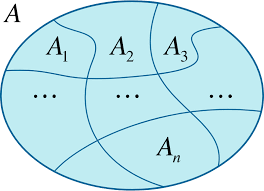
\includegraphics[scale=0.3]{partition.png}
\end{center}
Eine Partition einer Menge A ist eine Menge $\{A_i | i \in I\}$ von
paarweise disjunkten, nichtleeren Teilmengen von A mit
\begin{equation}
    \bigcup_{i \in I} A_i = A
\end{equation}
Die Elemente $A_i$ heissen die Klassen der Partition.werden auch deren Blöcke genannt.
\subsection{Beispiel}
Durch $A_0 = \{2n \mid n \in \mathbb{N}\}$ und $A_1 = \{2n+1 \mid n \in \mathbb{N}\}$ erhält
man eine Partition der natürlichen Zahlen in zwei unendlich grosse Blöcke.

\subsection{Induzierte Partition}
Folgt aus der Reflexivität einer Äquivalenzrelation und der
Äquivalenz:
\begin{equation}
    [a]_{\sim} = [b]_{\sim} \Leftrightarrow [a]_{\sim} \cap [b]_{\sim} \neq \emptyset
\end{equation}
\subsection{Induzierte Äquivalenzrelation}
Ist $P = \{A_i \mid i \in I \}$ eine Partition einer Menge A, dann ist die Relation $\sim$ mit\dots
\begin{equation}
    a \sim b \Leftrightarrow \exists{i} \in I(a \in A_i \wedge b \in A_i)
\end{equation}
...eine Äquivalenzrelation auf A.
\section{Unendliche Mengen}
Eine Menge $A$ ist nicht endlich, wenn $|A| = \infty$
\subsection{Abzählbare Mengen}
Eine Menga $A$ heisst abzählbar, wenn $A = \emptyset$ oder es eine der folgenden (äquivalenten)
Bedingungen erfüllt:
\begin{itemize}
	\item $|A| = |\N|$
	\item Es gibt eine surjektive Funktion $f: \N \twoheadrightarrow A$
	\item Es gibt eine injektive Funktion $g: A \hookrightarrow \N$
\end{itemize}
Beispiele sind:
\begin{itemize}
	\item $\{1,2,3\}$
	\item $\N$
	\item $\Z$
	\item $\Q$
	\item $\PR$
\end{itemize}
\subsection{Überabzählbare Mengen}
Überabzählbare Mengen sind nicht abzählbar.
Beispiele sind:
\begin{itemize}
	\item $\R$: reele Zahlen
	\item $\C$: komplexe Zahlen
	\item $\I$: imaginäre Zahlen
	\item $B(\infty)$: alle unendlichen Binärsequenzen
	\item $\poset(\N)$: Potenzmenge von $\N$
\end{itemize}
\subsection{Satz von Canton-Bernstein}
Für beliebige nichtleere Mengen $A$ und $B$ sind folgende Aussagen
äquivalent:
\begin{itemize}
	\item $|A| \leq |B| \wedge |B| \leq |A|$
	\item $|A| = |B|$
\end{itemize}
\subsubsection{Schubfachprinzip}
Aus $|A| > |B|$ und $|A| \neq |B|$ folgt $|B| \not\leq |A|$
\subsubsection{Definition von Dedekind}
Eine Menge $A$ ist genau dann unendlich, wenn es eine injektive und nicht surjektive Funktion
\\$f: A \hookrightarrow A$ gibt.
	\subsubsection{Hilberts Hotel}
	Eine Menga $A$ ist genau dann unendlich, wenn eine echte Teilmenge $B \subset A$ mit $|A| = |B|$ existiert.
\section{Die Peano Axiome}
\subsection{Axiom 1}
0 ist eine natürliche Zahl.
\subsection{Axiom 2}
Jede natürliche Zahl $k$ hat genau einen Nachfolger $k+1$, der wiederum eine natürliche Zahl ist.
\subsection{Axiom 3}
Die Zahl 0 ist die einzige natürliche Zahl, die kein Nachfolger ist.
\subsection{Axiom 4}
Jede natürliche Zahl ist Nachfolger von höchstens einer natürlichen Zahl.
\subsection{Axiom der vollständigen Induktion}
Ist $A(n)$ eine Eigenschaft (ein Prädikat), sodass...
\begin{itemize}
    \item \textbf{Induktionsverankerung (I.V.):} $A(0)$
    \item \textbf{Induktionsschritt (I.S.):} $\forall{n} \in \N (A(n) \Rightarrow A(n+1))$
\end{itemize} 
...dann gilt $\forall{n} \in \N (A(n))$

\section{Induktion}
Es sei $A(n)$ eine Eigenschaft von natürlichen Zahlen:

\begin{itemize}
    \item \textbf{Verankerung:} $A(n)$
    \item \textbf{Schritt:} $\forall n \in \mathbb{N} \quad \big(A(n) \implies A(n+1)\big)$
\end{itemize}
\textbf{Induktionsannahme:}
\begin{align*}
    \sum_{i=1}^n \frac{1}{i(i+1)} = \frac{n}{n+1}
\end{align*}
\textbf{Induktions-Verankerung (IV, $n=0$):}
\begin{align*}
    \sum_{i=1}^0 \frac{1}{i(i+1)} = 0 = \frac{0}{0+1}
\end{align*}

\textbf{Zu zeigen:}
\begin{align*}
    \sum_{i=1}^{n+1} \frac{1}{i(i+1)} = \textcolor{red}{\frac{n+1}{n+2}}
\end{align*}

\textbf{Induktions-Schritt (IS, $n \to n+1$)}
\begin{align*}
    &\sum_{i=1}^{n+1} \frac{1}{i(i+1)}\\
    &= \sum_{i=1}^n \frac{1}{i(i+1)} + \frac{1}{(n+1)((n+1)+1)} \\
    &= \frac{n}{n+1} + \frac{1}{(n+1)(n+2)} \\
    &= \frac{n(n+2) + 1}{(n+1)(n+2)} \\
    &= \frac{n^2 + 2n + 1}{(n+1)(n+2)} \\
    &= \frac{(n+1)^2}{(n+1)(n+2)} \\
    &= \textcolor{red}{\frac{n+1}{n+2}}
\end{align*}

\section{Rekursion}
\begin{itemize}
    \item \textbf{Verankerung:} $F(0) = c$
    \item \textbf{Schritt:} $F(n) = F(k+1) = G(\underbrace{F(k)}_{Selbsbezug},k)$
\end{itemize}
\textbf{Beispiel Expontenation von $\N$:}
\begin{align*}
    & F(0) = &x^0 = 1 \\
    & F(n) = &x^n \\
    & F(n+1) = &(F(n),n)\\
    & x^{n+1} = &F(n) \cdot n \\
    & x^{n+1} = &x^n \cdot n
\end{align*}


\section{Formale Aussagenlogik}

\subsection{Formale Definition}
Die Syntax der Aussagenlogik (= Menge aller aussagenlogischen Formeln) ist
durch $N(\{x_1,x_2,...\},\{and,or,not\})$ mit \dots
\begin{align*}
	and(A,B) := A \vee B  \\
	or(A,B) := A \wedge B \\
	not(A) := \neg A
\end{align*}
\dots gegeben.
\subsubsection{Beispiele}
\begin{itemize}
	\item $x_2$
	\item $((x_1 \wedge x_7) \vee (x_5 \wedge \neg x_0))$
	\item $\neg\neg\neg(x_3 \wedge \neg x_5)$
\end{itemize}
\subsection{Visualisierung}

\begin{align*}
	(x_1 \wedge x_7) \vee (x_5 \wedge \neg x_0)
\end{align*}

\begin{center}
	\begin{tikzpicture}
		[level distance=1.5cm,
			level 1/.style={sibling distance=4cm},
			level 2/.style={sibling distance=2cm}]
		\node {$\vee$}
		child {node {$\wedge$}
				child {node {$x_1$}}
				child {node {$x_7$}}
			}
		child {node {$\wedge$}
				child {node {$x_5$}}
				child {node {$\neg$}
						child {node {$x_0$}}
					}
			};
	\end{tikzpicture}
\end{center}
\subsection{Strukturelle Rekursion}
\begin{itemize}
    \item $\wedge = min()$
    \item $\vee = max()$
\end{itemize}
\begin{align*}
    \llbracket(x_1 \wedge x_2) \vee x_3\rrbracket_3(1, 1, 0) &= \max(\llbracket x_1 \wedge x_2\rrbracket_3(1, 1, 0), \llbracket x_3\rrbracket_3(1, 1, 0)) \\
    &= \max(\min(\llbracket x_1\rrbracket_3(1, 1, 0), \llbracket x_2\rrbracket_3(1, 1, 0)), 0) \\
    &= \max(\min(1, 1), 0) \\
    &= \max(1, 0) \\
    &= 1
\end{align*}
\subsection{Normalformen}
\subsubsection{Definition}
\begin{itemize}
\item $K_0 := D_0 := \{x_1, x_2 \ldots \} \cup \{\neg x_1, \neg x_2 \ldots \}$
\item $K_{n+1} := \{A_1 \wedge \cdots \wedge A_k \mid A_1 \ldots A_k \in D_n\}$
\item $D_{n+1} := \{A_1 \vee \cdots \vee A_k \mid A_1 \ldots A_k \in K_n\}$
\end{itemize}

\subsubsection{Beispiele}
\begin{itemize}
\item $(\neg x_1 \wedge x_2) \vee x_3 \in D_2$
\item $(\neg x_1 \vee x_2) \wedge (x_3 \vee x_1) \in K_2$
\end{itemize}

\subsubsection{Bemerkung}
Es gelten für alle $n \in \mathbb{N}$:
\begin{itemize}
\item $D_n \subsetneq K_{n+1} \cap D_{n+1}$
\item $K_n \subsetneq D_{n+1} \cap K_{n+1}$
\end{itemize}
\subsection{KNF und DNF}
\subsubsection{Definition}
Die Formeln in $K_2$ sind in \textbf{konjunktiver Normalform (KNF)}, die
Formeln in $D_2$ sind in \textbf{disjunktiver Normalform (DNF)}.
\subsubsection{Satz}
Zu jeder Formel $A$ existieren äquivalente Formeln $A_K$ in KNF und
$A_D$ in DNF.

\section{Teilbarkeitslehre}
\subsection{Teilbarkeitsrelation}
Für $x,y \in \Z$ definieren wir:
\begin{itemize}
	\item $y$ ist genau dann ein Vielfaches von $x$, wenn eine ganze Zahl $t \in \Z$
	      mit $y = t \cdot x$ existiert.
	\item $x$ ist genau dann ein Teiler $y$, wenn $y$ ein Vielfaches von $x$ ist.
	      Wenn $x$ ein Teiler von $y$ ist, dann schreiben wir $x|y$.
	\item Die Menga aller natrürlichen Teiler $T(x) := \{n \in \N | n|x\}$ von der Zahl $x$ besteht
	      aus allen natrürlichen Zahlen, die $x$ teilen.
\end{itemize}
\subsubsection{Beispiele}
\begin{itemize}
	\item $T(-4) = \{1,2,4\}$
	\item $T(1) = \{1\}$
	\item $T(0) = \N$
\end{itemize}
\subsection{Teilen mit Rest}
Sind $a,b \in \Z$ mit $b \neq 0$, dann gibt es höchstens ein Paar $(m,r) \in \Z^2$ mit:
\begin{itemize}
	\item $a = mb + r$
	\item $0 \leq r < |b|$
\end{itemize}
\subsection{Modulo Operator \& Ganzzahlige Division}
Die Funktion $mod : \Z \times \Z \ \{0\} \to \N$ und $div: \Z \times \Z \ \{0\} \to \Z$ sind so definiert
, dass \dots
\begin{align*}
	a = \text{div}(a,b) \cdot b + \text{mod}(a,b) \\
	0 \leq \text{mod}(a,b) < |b|
\end{align*}
\dots gilt. Die Funktion $mod$ nennt man Modulo Operator und die Funktion $div$ entspricht für  positive
Zahlen der ganzzahligen Division.
\subsubsection{Beispiele}
\begin{itemize}
	\item Es gilt $17 = 3 \cdot 5 + 2$ und daher $\text{div}(17, 5) = 3$ und
	      $\text{mod}(17, 5) = 2$.
	\item Es gilt $22 = -3 \cdot -7 + 1$ und daher $\text{div}(22, -7) = -3$ und
	      $\text{mod}(22, -7) = 1$.
	\item Es gilt $-22 = 4 \cdot -7 + 6$ und daher $\text{div}(-22, -7) = 4$ und
	      $\text{mod}(-22, -7) = 6$.
	\item Es gilt $-22 = -4 \cdot 7 + 6$ und daher $\text{div}(-22, 7) = -4$ und
	      $\text{mod}(-22, 7) = 6$.
\end{itemize}
\subsection{Grösster gemeinsamer Teiler}
Es seien $a,a_1, \dots,a_n$ beliebige ganze Zahlen.
\begin{itemize}
	\item $T(a_1, \dots,a_n) := T(a_1) \cap \cdots \cap T(a_n)$ ist die Menge aller gemeinsamer natrürlichen
	      Teiler der Zahlen $a_1, \dots,a_n$.
	\item $ggT(a_1, \dots,a_n) := \max(T(a_1, \dots,a_n))$ ist der grösste gemeinsame Teiler der Zahlen.
	      Eine der Zahlen muss jedoch von $0$ verschieden sein.
	\item Zwei ganze Zahlen $a,b$ heissen teilerfremd, wenn $ggT(a,b) = 1$ gilt.
\end{itemize}
\subsection{Euklidischer Algorithmus}
\subsection{Lemma}
Für beliebige ganze Zahlen $a,b$ gilt: \\$T(a,b) = T(a,b-a)$.
\subsubsection{Folgerung}
\begin{itemize}
	\item Für ganze Zahlen $a,b$ gilt: $ggT(a,b) = ggT(a,b-a)$.\\
	\item Für ganze Zahlen $b \geq a$, die nicht beide Null sind, gilt: \\$ggT(a,b) = ggT(a, mod(b,a))$
	      \\$ggT(a,b) = ggT(mod(a,b),b)$.
\end{itemize}
\subsubsection{Beispiel}
\begin{align*}
	 & ggT (25, 45) = ggT (25, mod(45, 25)) \\
	 & = ggT (25, 20)                       \\
	 & = ggT (mod(25, 20), 20)              \\
	 & = ggT (5, 20)                        \\
	 & = ggT (5, mod(20, 5))                \\
	 & = ggT (5, 0)                         \\
	 & = 5
\end{align*}
\subsection{Lemma von Bézout}
Sind $x,y \in \Z$ mit $(x,y) \neq (0,0)$, dann gibt es Zahlen $a,b$ sodass
\begin{align*}
	ggT(x,y) = ax + by
\end{align*}
gilt. Die Zahlen $a,b$ werden Bézout-Koeffizienten genannt.
\subsubsection{Beispiel}
\textbf{Gleichung:} 
\begin{align*}
    a \cdot 504 + b \cdot 29 = ggT(504,29) = 1
\end{align*}
\textbf{Schritt 1: Sukzessives Teilen mit Rest.}
\begin{align*}
	504 & = 17 \cdot 29 + 11                                \\
	29  & = 2 \cdot 11 + 7                                  \\
	11  & = 1 \cdot 7 + 4                                   \\
	7   & = 1 \cdot 4 + 3                                   \\
	4   & = 1 \cdot 3 + \underbrace{1}_{\text{ggT}(504,29)}
\end{align*}
\\
\textbf{Schritt 2: ``Rückwärts einsetzen''.}
\begin{align*}
	 & 1 = 4 - 3                                                                                      \\
	 & = (11-7) - (7-4)                                                                               \\
	 & = ((504-17 \cdot 29) - (29-2 \cdot 11))                                                        \\
     & \quad - ((29-2 \cdot 11) - (11-7))                                                                    \\
	 & = ((504-17 \cdot 29) - (29-2 \cdot (504-17 \cdot 29)))                                         \\
	 & \quad -((29-2 \cdot (504-17 \cdot 29))                                                       \\
     & \quad -((504-17 \cdot 29) - (29-2 \cdot (504-17 \cdot 29))))
\end{align*}
\\
\textbf{Schritt 3: Zusammenfassen (Zählen der Vorkommen von 504 und 29).}
\begin{align*}
	a & = 1 + 2 + 2 + 1 + 2 = 8                            \\
	b & = -17 - 1 - (2 \cdot 17) - 1 - (2 \cdot 17) = -139
\end{align*}
\\
\textbf{Test:}
\begin{align*}
    8 \cdot 504 - 139 \cdot 29 = 1
\end{align*}

\section{Primzahlen}
\subsection{Definition}
Eine natürliche Zahl $p \in \N$ ist eine Primzahl, wenn $|T(p)| = 2$ gilt. Die Menge aller Primzahlen
nennen wir $\PR$.\\\\
Eine natürliche Zahl $p > 1$ ist genau dann eine Primzahl, wenn
$T(p) = \{1, p\}$ gilt.
\subsection{Lemma von Euklid}
Die folgenden Aussagen sind für $p \in \N $ äquivalent.
\begin{enumerate}
    \item $p$ ist eine Primzahl.
    \item $\forall{n,m} \in \N (p|nm \Rightarrow p|n \vee p|m)$
\end{enumerate}
\subsection{Eindeutigkeit der Primfaktoren}
Sind $p_1, \ldots, p_m$ und $q_1, \ldots, q_n$ Primzahlen mit
\begin{align*}
    \prod_{i=1}^{m} p_i = \prod_{i=1}^{n} q_i
\end{align*}
dann gilt $n=m$ und $p_i = q_i$ für alle $0 \leq i \leq n$
\subsubsection{Folgerung}
Es sei $p_i$ jeweils die i-te Primzahl. Für jede natürliche Zahl $n > 1$
gibt es eine eindeutig bestimmte, endliche Folge $a_1, .., a_k$ von
natürlichen Zahlen mit $a_k \neq 0$, so dass
\begin{align*}
    n = \prod_{i=1}^{k} p_i^{a_i}
\end{align*}
gilt.
\section{Kongruenz Modulo}
\subsection{Definition}
\begin{itemize}
	\item Für $n \in \N$ und $r,s \in \Z$ gilt:
	      \begin{align*}
		      r \equiv_n s \Leftrightarrow n|(r-s)
	      \end{align*}
	\item Wir schreiben alternativ auch $r \equiv s \mod n$
	\item Für jede ganze Zahl $z$ bezeichnen wir mit
	      \begin{align*}
		      [z]_n := \{x \in \Z | x \equiv_n z\}
	      \end{align*}
	      die Äquivalenzklasse von $z$ bezüglich der Raltion $\equiv_n$ und nennen diese auch die \textbf{Restklasse} von $z$.
	\item Abkürzend bezeichnen wir $[z]_n$ auch mit $[z]$ oder $\overline{z}$, wenn $n$ aus
	      dem Kontext hervor geht.
\end{itemize}
\subsection{Rechnen mit Restklassen}
Für ganze Zahlen $x ,x'$ und $y, y'$ gelten
\begin{itemize}
	\item $[x] = [x'] \land [y] = [y'] \Rightarrow [x + y] = [x' + y']$
	\item $[x] = [x'] \land [y] = [y'] \Rightarrow [xy] = [x'y']$
\end{itemize}
\subsubsection{Addition und Multiplikation}
Die vorhergehende Bemerkung rechtfertigt die
Repräsentatnetnweise Definition der Multiplikation und Addition
auf Restklassen.
\begin{align*}
	 & + : \Z/n{^2} \to \Z/n \quad \mapsto \quad [x]_n + [y]_n := [x + y]_n             \\
	 & \cdot : \Z/n{^2} \to \Z/n \quad \mapsto \quad [x]_n \cdot [y]_n := [x \cdot y]_n \\
	 & \quad \text{wobei}                                                               \\
	 & \quad \Z/n = \Z/ \equiv_n = \{[0]_n, [1]_n, \ldots, [n-1]_n\}
\end{align*}
\textbf{Beispiele:}\\
\begin{itemize}
	\item $[17]_5 + [3]_5 = [20]_5 = [0]_5$
	\item $[2]_5 + [3]_5 = [5]_5 = [0]_5$
	\item $[17]_5 \cdot [3]_5 = [51]_5 = [1]_5$
	\item $[2]_5 \cdot [3]_5 = [6]_5 = [1]_5$
\end{itemize}
\subsection{Additive Inverse in $\Z/n$}
\subsubsection{Definition}
Sind $x,y \in \Z/n$, dann ist $x$ das additive Inverse von $y$, falls $x + y = [0]_n$ gilt.
\subsubsection{Beispiel}
In $\Z/7$ ist $[3]_7$ das additive Inverse von $[4]_7$, weil $[3]_7 + [4]_7 = [7]_7 = [0]_7$ gilt.
\subsubsection{$a + x = b$}
In $\Z/n$ gilt hat jedes Element ein additives Inverses, weswegen alle
Gleichungen von der Form $a + x = b$ mit $a,b \in \Z$ lösbar sind.\\\\
\textbf{Beispiel:}\\
In $\Z/7$ hat die Gleichung
\begin{align*}
	[3]_7 + x = [2]_7
\end{align*}
die Lösung $x = [2 + (7 - 3)]_7 = [6]_7$.
\subsection{Multiplikatives Inverse}
\subsubsection{Definition}
Sind $x, y \in \mathbb{Z}/n$, dann ist $x$ das \textbf{multiplikative Inverse}
von $y$, falls $x \cdot y = [1]_n$ gilt. Falls $x$ das multiplikative Inverse von $y$ ist, dann bezeichnen
wir $x$ auch als $y^{-1}$.

\subsubsection{Beispiel}
In $\mathbb{Z}/7$ ist $[3]_7$ das multiplikative Inverse von $[5]_7$,
weil $[3]_7 \cdot [5]_7 = [15]_7 = [1]_7$ gilt.
\subsection{Satz}
In $\Z/n$existiert genau dann ein multiplikatives Inverses zu $[x]$, wenn $ggT(n,x) = 1$ gilt,
Daraus folgt, dass in $\Z/n$ genau dann jedes Element ausser $[0]$ ein multiplikatives
Inverses, wenn $n$ eine Primzahl ist.

\section{Chinesischer Restsatz}
Sind $n_1, \ldots, n_k \in \N$ paarweise teilerfremd und $y_1, \ldots, y_k \in \Z$, dann
hat das Gleichungssystem
\begin{align*}
	x & \equiv_{n_1} y_1 \\
	x & \equiv_{n_2} y_2 \\
	  & \vdots           \\
	x & \equiv_{n_k} y_k
\end{align*}
eine eindeutige Lösung in $\Z/(n_1, \ldots,n_k)$.
\subsection{Lösen simultaner Kongruenzen}

Gegeben ein System simultaner Kongruenzen mit zwei Gleichungen:
\begin{align*}
	x & \equiv_{n_1} y_1 \\
	x & \equiv_{n_2} y_2
\end{align*}

\noindent wobei $n_1$ und $n_2$ teilerfremd sind.
\begin{enumerate}
	\item Bestimme mithilfe des Euklidischen Algorithmus Bézout Koeffizienten $a$ und $b$ mit $an_1 + bn_2 = 1$.
	\item Setze $x_0 := y_1bn_2 + y_2an_1$.
	\item Die resultierende Gleichung ist $x \equiv_{n_1 \cdot n_2} x_0$.
\end{enumerate}
\section{Beispiel}
\begin{align*}
    x & \equiv_7 3 \\
    x & \equiv_5 2 \\
    x & \equiv_9 6
\end{align*}
\subsection{Kleiner Fermat}
Ist $p \in \PR$ und $a$ kein Vielfaches von $p$, dann gilt:
\begin{align*}
    a^{p-1} \equiv_p 1
\end{align*}
%\section{Lemmas}
\subsection{Transitivität der Implikation}
Für alle Prädikate mit A,B und C mit \(A \Rightarrow B\) und \(B \Rightarrow C\) gilt \(A \Rightarrow C\).
\subsection{Kontraposition}
Für alle Prädikate mit A und B gilt \(A \Rightarrow B \Leftrightarrow \neg B \Rightarrow \neg A\).\\
Beweis. Wir wenden die Junktorenregeln an:\\
\begin{align*}
    A \Rightarrow B \\
    \Leftrightarrow \neg A \vee B && \text{Definition von A $\rightarrow$ B}\\
    \Leftrightarrow B \vee \neg A && \text{Kommutativität}\\
    \Leftrightarrow \neg\neg B \vee \neg A && \text{Doppelte Negation}\\
    \Leftrightarrow \neg B \Rightarrow \neg A && \text{Definition von $\neg B \rightarrow \neg A$}\\
\end{align*}
\subsection{Symetrie $\wedge$ Antisymetrie}
Es sei A eine beliegende Menge und R eine beliebige Relation. auf A. Die folgenden Aussagen sind äquivalent:\\
\begin{itemize}
    \item Die Relation R ist in der gleichheitsrelation auf A enthalten:\\ $G \subseteq \{(x,x) \mid x \in A\}$
    \item Die Relation R ist symetrisch und antisymetrisch.
\end{itemize}

\end{multicols*}
\end{document}